\label{chapter:isoperimetricinequality}
En este capítulo vamos a probar uno de los resultados más importantes de este trabajo: la desigualdad isoperimétrica en $\rtres$. Se trata de una relación funcional entre el área de una superficie compacta y conexa, y el volumen que ésta encierra. Su prueba está basada en la desigualdad de Brunn-Minkowski, que probaremos tras una serie de preliminares.

\section{Desigualdad de Brunn-Minkoski}

\begin{definition}[Suma conjuntista]
Si $A, B$ son dos conjuntos de $\rmath^n$, definimos la \textbf{suma conjuntista} $A+B$ como:

\begin{equation*}
    A+B = \{a+b \enspace | \enspace a \in A, b \in B\}.
\end{equation*}
\end{definition}

En los siguientes resultados se recogen algunas propiedades sencillas de la suma conjuntista.

\begin{lemma}
Sean $A,B \subseteq \rmath^n$. Si uno de los dos conjuntos es abierto, entonces la suma $A+B$ es un abierto.
\end{lemma}
\begin{proof}
Supongamos que $A$ es abierto. Nótese que:
\begin{equation*}
    A + B = \{a+b \enspace | \enspace a \in A, b \in B\} = \displaystyle\bigcup_{b \in B} \{a+b \enspace | \enspace a \in A\}
\end{equation*}

Como la unión de abiertos es abierta, luego solo nos falta ver que cada conjunto $\{a+b \enspace | \enspace a \in A\}$ es abierto.

En efecto, tenemos que el conjunto $\{a+b \enspace | \enspace a \in A\}$ es la traslación por el vector $b$ del conjunto $A$, que es un movimiento rígido y una aplicación abierta. Concluimos que $A+B$ es un abierto.

Análogo razonamiento sirve cuando $B$ abierto.
\end{proof}


\begin{lemma}
Sean $A,B \subseteq \rmath^n$. Si ambos conjuntos están acotados, entonces la suma $A+B$ está acotada.
\end{lemma}
\begin{proof}
La demostración de esta propiedad es consecuencia directa de la desigualdad triangular.

Sean $L,K > 0$ las cotas de $A$ y $B$ respectivamente. Así:
\begin{equation*}
    |a+b| \leq |a|+|b| \leq L + K, \qquad \forall a \in A, \forall b\in B
\end{equation*}

Luego $A+B$ está acotado.
\end{proof}

\begin{lemma}
Sean $A,B \subseteq \rmath^3$. Si ambos conjuntos son arco-conexos, entonces la suma $A+B$ es arco-conexo.
\end{lemma}
\begin{proof}
Veamos que $\forall c,d \in A+B$, $\exists \sigma: [0,1] \longrightarrow A+B$ arco, tal que $\sigma(0)=c$ y $\sigma(1)=d$.

Sean $c=a_1 + b_1$, $d=a_2+b_2$ cualesquiera pertenecientes a $A+B$. Por ser $A$ y $B$ arco-conexos, tenemos que existe un arco $\sigma_1: [0,1] \longrightarrow A$ con $\sigma_1(0)=a_1$ y $\sigma_1(1)=a_2$, y $\sigma_2: [0,1] \longrightarrow B$ con $\sigma_2(0)=b_1$ y $\sigma_2(1)=b_2$. Definiendo, $\sigma: [0,1] \longrightarrow A+B$ como $\sigma(t) = \sigma_1(t) + \sigma_2(t)$ tenemos un arco tal que $\sigma(0)=\sigma_1(0) + \sigma_2(0) = a_1+b_1 = c$ y $\sigma(1)=\sigma_1(1) + \sigma_2(1) = a_2+b_2 = d$.
\end{proof}

\begin{lemma}\label{paralelepipedoslemma}
Sean $I_1, I_2, I_3$ y $J_1, J_2, J_3$ intervalos abiertos de $\rmath$. Los subconjuntos de $\rtres$ dados por:
%
\begin{equation*}
    A = I_1 \times I_2 \times I_3, \qquad B = J_1 \times J_2 \times J_3
\end{equation*}
%
son llamados \textbf{paralelepípedos con los ejes paralelos a los ejes coordenados}. Entonces tenemos:
%
\begin{equation*}
    A + B = (I_1 + J_1) \times (I_2 + J_2) \times (I_3 + J_3)
\end{equation*}

Además, si $A$ y $B$ son disjuntos, tenemos que existe un plano paralelo a uno de los ejes coordenados que separan $A$ y $B$.
\end{lemma}
\begin{proof}
La igualdad sale directamente de la definición de suma conjuntista.
Veamos que si $A$ y $B$ son disjutos, entonces existe un plano paralelo a uno de los ejes coordenados que separan $A$ y $B$. Si $A \cap B = \emptyset$ entonces $I_i \cap J_i = \emptyset$ para al menos algún $i = 1,2,3$. Supongamos sin perder generalidad que se cumple para $i=1$, existe $a \in \rmath$ tal que los intervalos $I_1$ y $J_1$ están a lados distintos de $a$. Luego sea $x=a$ el plano que buscamos.
\end{proof}

Con estos preliminares, vamos a demostrar la desigualdad de Brunn-Minkowski seguiremos la demostración que aparece en la sección 6.5 de \cite{montielrosbook}.

\begin{theorem}[Desigualdad de Brunn-Minkowski]
Sean $A, B$ dos abiertos acotados del espacio euclídeo $\rtres$. Se cumple:

\begin{equation*}
    (vol \, A)^{\frac{1}{3}} + (vol \, B)^{\frac{1}{3}} \leq (vol \, (A+B))^{\frac{1}{3}}.
\end{equation*}
\end{theorem}
\begin{proof}
Esta demostración la vamos a realizar en tres pasos. Primero vamos a probar la desigualdad cuando $A,B$ son paralelepípedos. A continuación, cuando son unión finita de paralelepípedos abiertos, disjuntos y acotados cuyos lados son paralelos a los ejes coordenados. Finalmente, probaremos el caso de dos abiertos acotados cualesquiera.

Supongamos primero el caso de paralelepípedos $A = I_1 \times I_2 \times I_3$ y $B = J_1 \times J_2 \times J_3$, donde $I_i,J_i$ son intervalos abiertos y acotados de $\rmath \quad \forall i=1,2,3$ de longitudes $a_i$ y $b_i \quad \forall i=1,2,3$. Luego:
%
\begin{equation*}
    \frac{ \left(vol \, A \right)^{1/3} + \left(vol \, B \right)^{1/3}}{\left(vol \, (A+B) \right)^{1/3}} = \frac{\left(\displaystyle\prod_{i=1}^3 a_i \right)^{1/3} + \left(\displaystyle\prod_{i=1}^3 b_i \right)^{1/3}}{\left(\displaystyle\prod_{i=1}^3 (a_i+b_i) \right)^{1/3}},
\end{equation*}
%
y, por tanto:
%
\begin{equation*}
    \frac{ \left(vol \, A \right)^{1/3} + \left(vol \, B \right)^{1/3}}{\left(vol \, (A+B) \right)^{1/3}} = \left(\displaystyle\prod_{i=1}^3 \frac{a_i}{a_i+b_i} \right)^{1/3} + \left(\displaystyle\prod_{i=1}^3 \frac{b_i}{a_i+b_i} \right)^{1/3}
\end{equation*}
%
Además, por la desigualdad de las medias, sabemos que:
%
\begin{equation*}
    \frac{ \left(vol \, A \right)^{1/3} + \left(vol \, B \right)^{1/3}}{\left(vol \, (A+B) \right)^{1/3}} \leq
    \frac{1}{3} \displaystyle\sum_{i=1}^3 \frac{a_i}{a_i+b_i} + \frac{1}{3} \displaystyle\sum_{i=1}^3 \frac{b_i}{a_i+b_i} = 1.
\end{equation*}
%
Para este caso la desigualdad queda probada.

Supongamos ahora el segundo caso; sean $A = \displaystyle\bigcup_{i=1}^n A_i$ y $B = \displaystyle\bigcup_{j=1}^m B_j$ (uniones disjuntas) donde $A_i$, $B_j$ son paralelepípedos como los del primer caso.

Vamos a probar la desigualdad por inducción sobre el número total de paralelepípedos, $t = n + m$.
El caso $t=2$ es claro, pues es el caso previamente demostrado.
Supongamos cierta la desigualdad cuando $t < n + m$ y veamos que es cierta para $t \geq n + m$. Como ya hemos visto que $t=2$ es cierto, podemos suponer que $n + m \geq 3$ luego es claro que $n > 1$ or $m > 1$.

Supongamos $n > 1$. Por el lema \ref{paralelepipedoslemma} tenemos que existe un plano $P$ separando $A_1$ y $A_2$. Sea $P^+$ y $P^-$ los dos semiespacios abiertos en los que $P$ divide a $\rtres$, y sean $A^+ = A \cap P^+$ y $A^- = A \cap P^-$. Podemos expresar:

\begin{equation*}
    A^+ = \displaystyle\bigcup_{i=1}^{n^+} A_i^+, \qquad A^- = \displaystyle\bigcup_{i=1}^{n^-} A_i^-,
\end{equation*}

que son uniones finitas de paralelepípedos cuyos ejes son paralelos a los ejes coordenados. Además $n^+ < n$ y $n^- < n$ ya que $P$ separa al menos a $A_1$ y $A_2$.

Por otro lado, existe un plano $Q$ paralelo a $P$ que cumple:

\begin{equation}\label{equationvolumen}
    \frac{vol \, A^+}{vol \, A} = \frac{vol \, B^+}{vol B}.
\end{equation}

Esto es posible ya que $\frac{vol A^+}{vol \, A} = c$ con $0 < c < 1$. Luego podemos tomar $Q$ a la izquierda de todos los paralelepípedos de $B$ y desplazarlo a la derecha hasta encontrar la igualdad, gracias a que $\frac{vol \, B^+}{vol \, B}$ es una función continua, vease la \autoref{fig:brunninequality}.
Dado que $vol A = vol \, A^+ + vol \, A^-$ y $vol \, B = vol B^+ + vol \, B^-$ tenemos la misma \autoref{equationvolumen} para $A^-$ y $B^-$.

\begin{figure}[h]
  \centering
  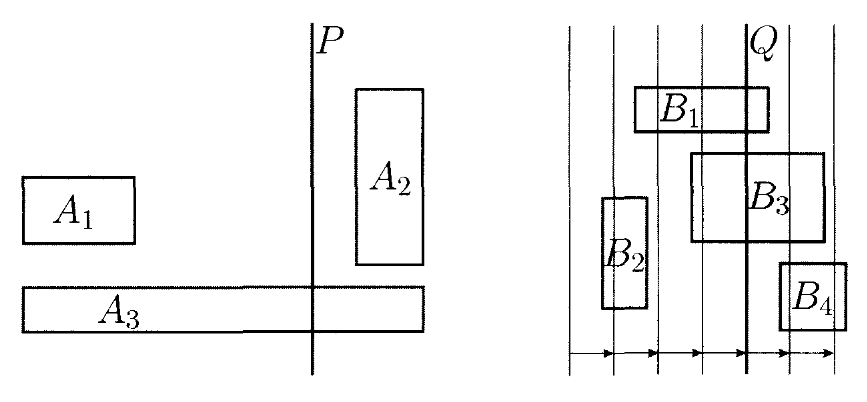
\includegraphics[width=0.9\textwidth]{gfx/brunninequality.png}
  \caption{\label{fig:brunninequality}Elección de $P$ y $Q$. Imagen obtenida de \cite{montielrosbook}.}
\end{figure}

Al igual que ocurre con $A$, tenemos que 
%
\begin{equation*}
    B^+ = \displaystyle\bigcup_{j=1}^{m^+} B_j^+, \qquad B^- = \displaystyle\bigcup_{j=1}^{m^-} B_j^-,
\end{equation*}
%
con $m^+ \leq m$ y $m^- \leq m$. En este caso, no podemos suponer que $m^+ < m$ y $m^- < m$ debido a que no tenemos garantizado el hecho de que $Q$ separe a dos paralelepípedos de $B$.

Estamos en condiciones de aplicar la hipótesis de inducción a los pares $A^+$, $B^+$ y $A^-$, $B^-$ ya que el total de paralelepípedos cumple la condición $n^+ + m^+ < n + m$ y $n^- + m^- < n + m$. Por tanto tenemos:

\begin{equation*}
    vol \, (A^+ + B^+) \geq \left[ (vol \, A^+)^{1/3} + (vol \, B^+)^{1/3} \right]^3
\end{equation*}
\begin{equation*}
    vol \, (A^- + B^-) \geq \left[ (vol \, A^-)^{1/3} + (vol \, B^-)^{1/3} \right]^3
\end{equation*}

Por otro lado, como $A^+ \subset P^+$ y $B^+ \subset Q^+$, entonces $A^+ + B^+ \subset P^+ + Q^+$ y análogamente $A^- + B^- \subset (P+Q)^-$. Teniendo en cuenta que $P+Q$ es otro plano de $\rtres$ tenemos que $A^+ + B^+$ y $A^- + B^-$ son disjuntos. En consecuencia:
%
\begin{align*}
    vol \, (A+B) &\geq vol \,(A^+ + B^+) + vol \,(A^- + B^-) \\ 
    &\geq \left[ (vol \, A^+)^{1/3} + (vol \, B^+)^{1/3} \right]^3 + \left[ (vol \, A^-)^{1/3} + (vol \, B^-)^{1/3} \right]^3
\end{align*}

Teniendo en cuenta la \autoref{equationvolumen} y su análoga para $A^-$ y $B^-$, se sigue que:
%
\begin{align*}
    vol \, (A+B) &\geq vol \, A^+ \left[ 1 + \left( \frac{vol \, B}{vol \, A} \right)^{1/3}  \right]^3 + vol \, A^- \left[ 1 + \left( \frac{vol \, B}{vol \, A} \right)^{1/3}  \right]^3 \\
    &\geq vol \, A \left[ 1 + \left( \frac{vol \, B}{vol \, A} \right)^{1/3}  \right]^3 = \left[ (vol \, A)^{1/3} + (vol \, B)^{1/3} \right]^3,
\end{align*}
%
con lo que la desigualdad se cumple para este segundo caso.

Consideremos finalmente el tercer caso, con $A$ y $B$ dos abiertos acotados cualesquiera de $\rtres$. Usando la teoría de integración de Lebesgue, existen dos sucesiones de conjuntos abiertos de $\rtres$ como los del caso anterior $A_n$ y $B_n$, con $n \in \nmath$, tales que $A_n \subset A$, $B_n \subset B$ y:
%
\begin{equation*}
    \lim_{x \to \infty} vol \, A_n = vol \, A \qquad \lim_{x \to \infty} vol \, B_n = vol \, B
\end{equation*}

Luego tenemos que $A_n + B_n \subset A + B$ para cada $n \in \nmath$ y, por tanto:
%
\begin{equation*}
    vol \, (A+B)^{1/3} \geq vol \, (A_n+B_n)^{1/3} \geq vol \, (A_n) ^{1/3} + vol \, (B_n)^{1/3}, \qquad \forall n \in \nmath
\end{equation*}

Basta con tomar límites con $n$ tendiendo a infinito y tenemos probada la desigualdad para todos los casos.
\end{proof}

\section{La desigualdad isoperimétrica en $\rtres$}

Con la desigualdad de Brunn-Minkowski demostrada, vamos a probar el resultado más importante de este capítulo.
\begin{theorem}[Desigualdad Isoperimétrica]
Sea $S$ una superficie conexa y compacta con dominio interior $\Omega$. Se cumple:

\begin{equation*}
    A(S)^3 \geq 36\pi(vol \, \Omega)^2.
\end{equation*}
\end{theorem}
\begin{proof}
Para demostrarlo, tenemos que buscar primero cierta situación donde podamos aplicar la desigualdad de Brunn-Minkowski.

Tomamos $\epsilon > 0$ tal que $N_\epsilon(S)$ es un entorno tubular. Para cada $t \in (0, \epsilon)$, sea $S_t$ la correspondiente superficie paralela incluida en $\Omega$ y $\Omega_t$ el dominio interior determinado por $S_t$. Además, vamos a tomar $B_t$ como la bola abierta centrada en el origen de $\rtres$ y radio $t$.

Consideremos el conjunto $\Omega_t + B_t$, $\forall t \in (0, \epsilon)$. Veamos primero que $(\Omega_t + B_t) \cap S = \emptyset$. Sea $p \in (\Omega_t + B_t) \cap S$. Por definición, $p = q + v$ con $q \in \Omega_t$ y $v \in B_t$, luego se cumple que $|p - q| = |v| < t$, luego $dist(q, S) < t$. Esto es una contradicción ya la distancia de $q$ a $S$ se alcanza en un punto $p_0$ tal que $q$ está en la recta normal de $p_0$ en $S$. Como $q \in \Omega_t$, tenemos que $|p_0 - q| \geq t$.

Por tanto, concluimos que $(\Omega_t + B_t) \cap S = \emptyset$. Por otro lado, sabemos que $\Omega_t$ y $B_t$ son arco-conexos, y hemos probado que la suma de arco-conexos es arco-conexa, por lo que $\Omega_t + B_t$ es arco-conexo y, por tanto, tiene que estar incluido en una de las componentes arco-conexas de $\rmath - S$. Teniendo en cuenta que $\Omega_t \subset \Omega$, tenemos que $\Omega_t + B_t \subset \Omega$, $\forall t \in (0, \epsilon)$.

Aplicando ahora la ya conocida desigualdad de Brunn-Minkowski, tenemos que:
%
\begin{equation*}
    vol \, \Omega \geq vol \, (\Omega + B_t) \geq \left[ (vol \, \Omega)^{1/3} + vol \, (B_t)^{1/3} \right]^3, \qquad \forall t \in (0, \epsilon).
\end{equation*}
%
desarrollamos la parte de la derecha y obtenemos:
%
\begin{equation*}
    vol \, \Omega \geq vol \, \Omega_t + 3(vol \, \Omega_t)^{2/3}(vol \, B_t)^{1/3} + vol \, B_t
\end{equation*}
%
y simplificando:
%
\begin{equation*}
    vol \, \Omega \geq vol \, \Omega_t + 3(vol \, \Omega_t)^{2/3}(vol \, B_t)^{1/3}
\end{equation*}

Sustituimos ahora el valor del volumen de la bola que hemos visto previamente:
%
\begin{align*}
    vol \, \Omega &\geq vol \, \Omega_t + 3(vol \, \Omega_t)^{2/3} \left( \frac{4\pi}{3}t^3 \right)^{1/3} \\
    vol \, \Omega &\geq vol \, \Omega_t + 3t \left( \frac{4\pi}{3} \right)^{1/3} (vol \, \Omega_t)^{2/3}
\end{align*}
%
y obtenemos:
%
\begin{equation*}
    \frac{vol \, \Omega - vol \, \Omega_t}{t} \geq 3 \left( \frac{4\pi}{3} \right)^{1/3} (vol \, \Omega_t)^{2/3}
\end{equation*}

Conociendo ahora el volumen encerrado entre superficies paralelas calculado en la \autoref{volumeparallelsurface}, nos queda:

\begin{equation*}
    \frac{tA(S) - t^2\int_S H \, dS + \frac{t^3}{3}\int_S K \, dS}{t} \geq 3 \left( \frac{4\pi}{3} \right)^{1/3} (vol \, \Omega_t)^{2/3},
\end{equation*}
%
es decir:
%
\begin{equation*}
    A(S) - t\int_S H \, dS + \frac{t^2}{3}\int_S K \, dS \geq 3 \left( \frac{4\pi}{3} \right)^{1/3} (vol \, \Omega_t)^{2/3}, \qquad \forall t \in (0,\epsilon).
\end{equation*}

Tomando límites en ambos lados con $t$ tendiendo a $0$, tenemos:
%
\begin{equation*}
    A(S) \geq 3 \left( \frac{4\pi}{3} \right)^{1/3} (vol \, \Omega)^{2/3},
\end{equation*}
%
y elevando al cubo tenemos la desigualdad que buscamos:

\begin{equation*}
    A(S)^3 \geq 36\pi(vol \, \Omega)^2.
\end{equation*}
\end{proof}

\begin{definition}[Superficie isoperimétrica]
Sea $S \subset \rtres$ una superficie compacta y conexa, $\Omega$ el dominio interior encerrado por $S$, $A(S)$ el área de $S$ y $vol \, \Omega$ el volumen de $\Omega$. Diremos que $S$ es una \textbf{superficie isoperimétrica} si para cada superficie $S'$ compacta y conexa con $\Omega'$ el dominio interior encerrado por $S'$ tal que $vol \, \Omega' = vol \, \Omega$ se cumple que $A(S) \leq A(S')$.
\end{definition}

\begin{proposition}\label{prop:spheresasisoperimetricsurfaces}
Las esferas son superficies isoperimétricas.
\end{proposition}
\begin{proof}
Veamos en primer lugar que las esferas cumplen la igualdad en la desigualdad isoperimétrica.

Sea $S=\unitsphere(p_0,r)$ superficie compacta y conexa y $\Omega = B(p_0,r)$ el dominio interior determinado por $S$. Sabemos que $A(S)=4\pi r^2$ y $vol \, \Omega = \frac{4\pi r^3}{3}$. A partir de aquí es inmediato comprobar que los dos términos que aparecen en la desigualdad isoperimétrica coinciden con $64\pi^3r^6$:

Veamos ahora que $S$ es una superficie isoperimétrica. Sea $S'$ otra superficie conexa y compacta tal que $vol \, \Omega' = vol \, \Omega$, donde $\Omega'$ es el dominio interior determinado por la superficie $S'$. Aplicando la desigualdad isoperimétrica:
%
\begin{equation*}
    A(S')^3 \geq 36\pi (vol \,)^2 = 36\pi (vol \, \Omega)^2 = A(S)^3 
\end{equation*}
%
donde en la última igualdad hemos usado que $S$ cumple la igualdad en la desigualdad isoperimétrica.
\end{proof}

\begin{corolario}\label{cor2}
Sea $S \subset \rtres$ una superficie compacta y conexa, y $\Omega$ su dominio interior. Entonces $S$ es isoperimétrica si y solo si $A(S)^3 = 36\pi (vol \, \Omega)^2$.
\end{corolario}
\begin{proof}
Vamos a probarlo por doble implicación. Veamos primero que si $S$ es una superficie isoperimétrica, entonces se cumple la igualdad.

Supongamos lo contrario e intentemos llegar a contradicción. Sea $S$ es una superficie isoperimétricas tal que $A(S)^3 > 36\pi (vol \, \Omega)^2$. Tomamos una esfera $S'$ tal que su volumen interior $\Omega'$ cumple $vol \, \Omega = vol \, \Omega'$. Como las esferas dan la igualdad en la desigualdad isoperimétrica, tendríamos:
%
\begin{equation*}
    A(S)^3 > 36\pi (vol \, \Omega)^2 = 36\pi (vol \, \Omega')^2 = A(S')^3,
\end{equation*}
%
con lo que $A(S') < A(S)$ y habríamos probado que $S'$ encierra el mismo volumen con menor área, por lo tanto $S$ no sería isoperimétrica y llegamos a contradicción.

Veamos ahora la otra implicación. Partimos de la suposición de que $S$ es una superficie tal que $A(S)^3 = 36\pi (vol \, \Omega)^2$ y queremos ver que es isoperimétrica.

Dada una superficie compacta y conexa $S'$ con $vol \, \Omega' = vol \, \Omega$, por la desigualdad isoperimétrica tenemos que:
%
\begin{equation*}
    A(S')^3 \geq 36\pi (vol \, \Omega')^2 = 36\pi(vol \, \Omega)^2 = A(S)^3,
\end{equation*}
%
luego
%
\begin{equation*}
    A(S) \leq A(S'),
\end{equation*}
%
y concluimos que $S$ es una superficie isoperimétrica.
\end{proof}

\paragraph{Nota}{En la proposición \ref{prop:spheresasisoperimetricsurfaces} hemos probado que las esferas minimizan el área entre todas las superficies conexas y compactas que encierran un volumen dado. Con argumentos similares se puede probar también que las esferas maximizan el volumen entre todas las superficies conexas y compactas de área dada.}

\paragraph{Nota}{La desigualdad de Brunn-Minkowski que hemos probado admite una extensión a $\rmath^n$ que se demuestra con los mismos argumentos. En concreto, si $A,B \subset \rmath^n$ son abiertos y acotados, entonces se cumple que:
\begin{equation*}
    (vol \, A)^{\frac{1}{n}} + (vol \, B)^{\frac{1}{n}} \leq (vol \, (A+B))^{\frac{1}{n}}.
\end{equation*}
%
Una prueba detallada puede encontrarse en el capítulo 2 de \cite{geometricinequalities}.
Como consecuencia, puede probarse en $\rmath^n$ un resultado análogo a la proposición \ref{prop:spheresasisoperimetricsurfaces}: las esferas de $\rmath^n$ minimizan el área (n-$1$)-dimensional entre todas las hipersuperficies conexas y compactas que encierran un volumen dado.}
